\chapter{2026}
\section*{一、程序阅读题}

1. 下面代码是关于深度优先生成树，请填写完整代码。图的邻接表存储结构及功能函数如下：

\begin{lstlisting}[language=C, basicstyle=\ttfamily]
typedef int VertexType; // 顶点数据类型

typedef struct ArcNode {  // 边表结点
    int adjvex;           // 该弧所指向的顶点位置
    struct ArcNode *nextarc; // 下个结点
} ArcNode;

typedef struct VNode {        // 顶点表结点
    VertexType data;          // 顶点信息
    ArcNode *firstarc;        // 指向第一条依附该顶点的弧的指针
} VNode;

typedef struct {              // 图
    VNode vertices[MaxVertexNum]; // 邻接表
    int vexnum, arcnum;       // 图的当前顶点数,图的边数/弧数
} ALGraph;

void DFS_Tree(ALGraph G)
{
    for(int i=0; i<G.vexnum; i++)
        visited[i] = false;
    for(int i=0; i<G.vexnum; i++)
        if(!visited[i])
            DFSTree(G, i);
}

void DFSTree(ALGraph G, int v)
{
    visited[v] = true;
    ArcNode *p = _____(1)_____;
    while(p != NULL)
    {
        if(!visited[p->adjvex])
        {
            printf("Tree edge:\%d \%d\n", v, p->adjvex);
            _____(2)_____;
        }
        p = p->nextarc;
    }
}
\end{lstlisting}

2. 给定一个共享栈，栈大小为 m，栈 1 的初始栈顶指针 top[0] 值初始指向 -1，栈 2 的初始栈顶指针 top[1] 值初始指向 m，请填写完整代码。共享栈存储类型可以描述为（题目中未给出该部分存储结构）：

\begin{lstlisting}[language=C, basicstyle=\ttfamily]
typedef struct
{
    int data[MaxSize];
    int top[2];  // 栈顶指针
    int bot[2];  // 栈尾指针
} TwStack;
\end{lstlisting}

初始化、入队和出队操作函数如下：

\begin{lstlisting}[language=C, basicstyle=\ttfamily]
void InitStack(TwStack &S)
{
    S.bot[0] = -1;
    S.bot[1] = m;
    S.top[0] = -1;
    S.top[1] = m;
}

bool Push(TwStack &S, int i, int x)
{
    if(_____(1)_____)
        return false;
    if(i == 0)
        S.data[_____(2)_____] = x;
    else if(i == 1)
        S.data[_____(3)_____] = x;
    return true;
}

bool Pop(TwStack &S, int i, int &x)
{
    if(S.top[i] == S.bot[i])
        return false;
    if(i == 0)
        x = S.data[_____(4)_____];
    else if(i == 1)
        x = S.data[_____(5)_____];
    return true;
}
\end{lstlisting}

\newpage

3. 假设有两个带头结点线性表 A 和 B，它们的元素都是依值递增有序排列，并且分别表示两个集合，现要求另辟空间构成一个线性表 C，其元素为 A 和 B 中元素的交集，且表 C 中的元素也依值递增有序排列。借助线性表 A 空间存放线性表 C，请填写完整代码。

\begin{lstlisting}[language=C, basicstyle=\ttfamily]
Status merge_list(LinkList &A, LinkList &B)
{
    LNode *pa = A->next;
    LNode *pb = B->next;
    LNode *pc = A;
    LNode *temp;

    while(_____(1)_____)
    {
        if(pa->data == pb->data)
        {
            _____(2)_____;
            pc = pa;
            pa = pa->next;
            temp = pb;
            pb = pb->next;
            free(temp);
        }
        else if(pa->data < pb->data)
        {
            temp = pa;
            pa = pa->next;
            free(temp);
        }
        else
        {
            temp = pb;
            pb = pb->next;
            free(temp);
        }
    }

    while(pb)
    {
        temp = pb;
        pb = pb->next;
        free(temp);
    }

    while(pa)
    {
        temp = pa;
        pa = pa->next;
        free(temp);
    }
    _____(3)_____;
    free(B);
    return OK;
}
\end{lstlisting}

4. 分析下列程序的输出结果，并给出算法的时间复杂度，其中 n 为 8。

\begin{lstlisting}[language=C, basicstyle=\ttfamily]
int a[] = {23, 33, 16, 79, 34, 79, 29, 86};

void riddle1(int n)
{
    if(n == 1)
        return;
    riddle1(n-1);
    if(a[n-1] < a[n-2])
        printf("%d ", a[n-1]);
    else
        printf("%d ", a[n-2]);
}

int riddle2(int n)  // 两函数不确定是哪个
{
    if(n == 1)
        return a[0];
    int p = riddle2(n-1);
    if(p < a[n])
        return p;
    else
        return a[n];
}
\end{lstlisting}

\newpage

5. 下面的代码是判断一个二叉树是否为平衡二叉树，若是平衡二叉树通过参数 depth 返回树的深度，并返回 true；若不是平衡二叉树，则返回 false，此时 depth 的值无意义。请填写完整代码。

二叉树的链式存储结构描述如下：

\begin{lstlisting}[language=C, basicstyle=\ttfamily]
typedef struct BiTNode {
    ElemType data;
    struct BiTNode *lchild, *rchild;
} BiTNode, *BiTree;
\end{lstlisting}

判断平衡二叉树函数如下：

\begin{lstlisting}[language=C, basicstyle=\ttfamily]
bool isBalanced(BiTree T, int &depth)
{
    if(T == NULL)
    {
        depth = 0;
        return true;
    }
    int deepleft, deepright;

    if(_____(1)_____)
    {
        int dif = deepleft - deepright;
        if(_____(2)_____)
        {
            depth = (deepleft > deepright ? deepleft : deepright) + 1;
            return true;
        }
    }
    return false;
}
\end{lstlisting}

\section*{二、填空题}

6. 已知 a=2, b=3, c=4, d=5，求出后缀表达式 abc*+d- 的计算值为\_\_\_\_\_\_\_\_\_\_。

7. 若用一个大小为 5 的数组来实现循环队列，且当前 front 和 rear 的值分别是 0 和 3，从队列中进队 1 次，出队 2 次后，front 和 rear 的值分别是\_\_\_\_\_\_\_\_\_\_。

8. 二维数组 A 按行优先存储，每个元素占 1 个空间，若 A[0][0] 的地址为 100，A[3][3] 地址为 220，则 A[5][5] 的地址为\_\_\_\_\_\_\_\_\_\_。

9. 栈按 1 到 n 依次进栈，出队序列为 \(T_{1},T_{2},\dots,T_{n}\)，若 \(T_{1}\) 为 n，则第 i 个出队的元素是\_\_\_\_\_\_\_\_\_\_。

10. 含有 n 个顶点的强连通图，边数至少为\_\_\_\_\_\_\_\_\_\_。

11. 含有 n 个结点的二叉树，在二叉链表中的空指针个数为\_\_\_\_\_\_\_\_\_\_。

12. 若长度为 n 的线性表采用链式存储结构，在其第 i 个位置插入一个元素的时间复杂度为\_\_\_\_\_\_\_\_\_\_。

13. 含 125 个元素的数组，折半查找成功的最多比较次数为\_\_\_\_\_\_\_\_\_\_。

14. 已知广义表 A = (a,b,(c,d),(e,(f,g)))，则 Head(Tail(Head(Tail(Tail(A))))) 的值为\_\_\_\_\_\_\_\_\_\_。

15. 无原题。下面是 AI 生成的类似的题目：给定一个大根堆 [9,6,8,3,4,5,7]，当插入元素 10 后，大根堆经过调整后，需要的比较次数为\_\_\_\_\_\_\_\_\_\_。

\begin{figure}[htbp]
    \centering
    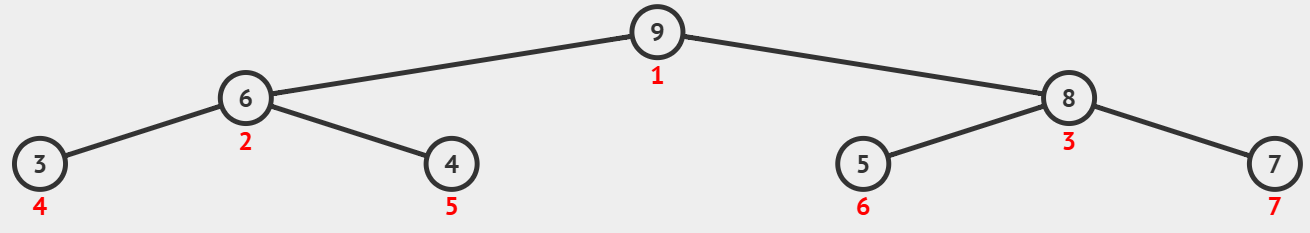
\includegraphics[width=0.3\textwidth]{images/2026/blank_15.png}
    \caption*{图1 15题图}
\end{figure}

\section*{三、综合应用题}
（回忆版综合应用题的序列、图不一定与考试一致，综合题顺序不一定一致）

16. 已知某二叉树的先序序列为 ABCDEFG，中序序列为 BADCFEG。

(1) 画出该二叉树，并给出该二叉树的后序序列；

(2) 画出该二叉树的三叉链表结构；

(3) 画出该二叉树对应的树或森林。

\vspace{10em}

17. 有一个散列表（也称哈希表）的散列函数为 H(key) = key \% 13，将关键字序列 19,14,23,1,68,20,84,27,55,11,10,79 按顺序插入空的哈希表：

(1) 若采用线性探测法处理冲突，请画出插入完成的哈希表，并求等概率下查找成功和查找失败时的平均查找长度，注意哈希表为 HT[0,\dots,15]，表长为 16。

(2) 若采用链地址法处理冲突，请画出插入完成的哈希表，并求等概率情况下查找成功和查找失败时的平均查找长度。

\vspace{10em}

\newpage

18. 给定一个整数序列 \{14,4,39,28,16,2,10,78\}

(1) 画出依次插入二叉排序树的最终形态；

(2) 计算查找成功的平均查找长度；

(3) 若一开始插入时进行平衡调整，给出最终的平衡二叉树的形态。

\vspace{10em}

19. 给定一个有向图，利用 Dijkstra 算法寻找从 V1 作为源点的最短路径。

\begin{figure}[htbp]
    \centering
    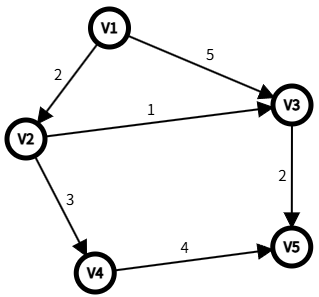
\includegraphics[width=0.3\textwidth]{images/2026/comprehensive_19_1.png}
    \caption*{图2 19题图1}
\end{figure}
\begin{figure}[htbp]
    \centering
    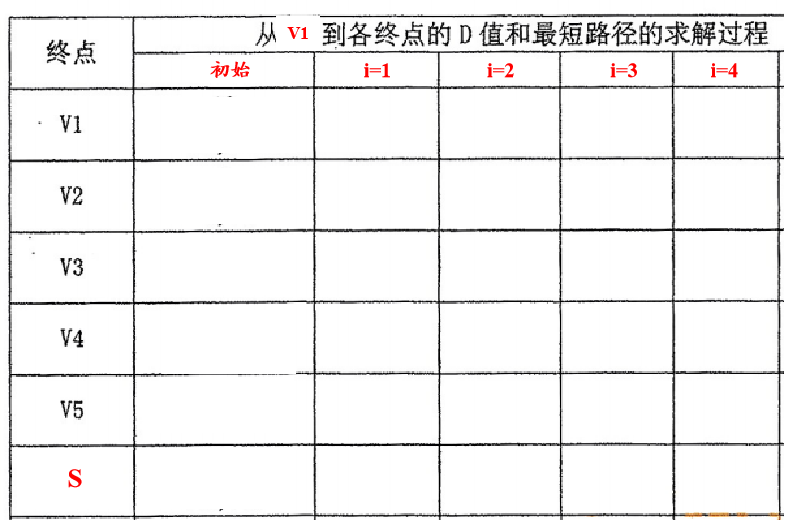
\includegraphics[width=0.3\textwidth]{images/2026/comprehensive_19_2.png}
    \caption*{图3 19题图2}
\end{figure}

\newpage

20. 给定一个 AOE 网，完成表格，要求给出计算过程，并给出关键路径。

\begin{figure}[htbp]
    \centering
    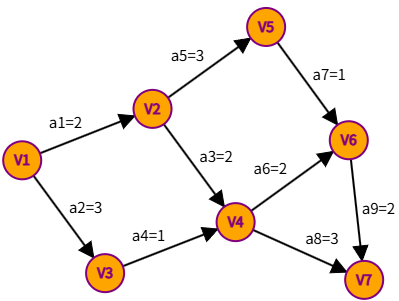
\includegraphics[width=0.3\textwidth]{images/2026/comprehensive_20.png}
    \caption*{图4 20题图}
\end{figure}

\begin{center}
\begin{tabular}{|c|c|c|c|c|c|c|c|}
\hline
事件 & V1 & V2 & V3 & V4 & V5 & V6 & V7 \\
\hline
最早发生时间 & \phantom{X} & \phantom{X} & \phantom{X} & \phantom{X} & \phantom{X} & \phantom{X} & \phantom{X} \\
\hline
最迟发生时间 & \phantom{X} & \phantom{X} & \phantom{X} & \phantom{X} & \phantom{X} & \phantom{X} & \phantom{X} \\
\hline
\end{tabular}
\end{center}

\vspace{2em}

\begin{center}
\begin{tabular}{|c|c|c|c|c|c|c|c|c|c|}
\hline
活动 & a1 & a2 & a3 & a4 & a5 & a6 & a7 & a8 & a9 \\
\hline
最早开始时间 & \phantom{X} & \phantom{X} & \phantom{X} & \phantom{X} & \phantom{X} & \phantom{X} & \phantom{X} & \phantom{X} & \phantom{X} \\
\hline
最迟开始时间 & \phantom{X} & \phantom{X} & \phantom{X} & \phantom{X} & \phantom{X} & \phantom{X} & \phantom{X} & \phantom{X} & \phantom{X} \\
\hline
\end{tabular}
\end{center}

\vspace{10em}

\newpage

21. 已知字母 a\(\sim\)g 的频率如下表所示。

(1) 采用赫夫曼（Huffman）编码算法对上述序列编码，给出相应的 Huffman 树，要求同一结点的左根大于右根；

(2) 对每个字母给出对应的编码，左 0 右 1，完成下表。

\begin{center}
\begin{tabular}{|c|c|c|c|c|c|c|c|}
\hline
字符 & a & b & c & d & e & f & g \\
\hline
出现频率 & 5 & 9 & 12 & 13 & 16 & 45 & 6 \\
\hline
编码 & \phantom{X} & \phantom{X} & \phantom{X} & \phantom{X} & \phantom{X} & \phantom{X} & \phantom{X} \\
\hline
\end{tabular}
\end{center}

\vspace{10em}

22. 给定有序序列 \{2,7,8,10,24,25,28,31,33,39,41\}

(1) 画出折半查找判定树；

(2) 查找元素 28 需要依次比较哪些元素；

(3) 在相等查找概率情况下，计算查找成功的平均查找长度。

\vspace{10em}

\newpage

23. 已知整数序列 \{46,79,56,38,40,84,29,10,15,37\}

(1) 将该序列建立初始小根堆，并写出最终形态的小根堆；

(2) 使用二路归并排序对原序列进行升序排序，写出每趟归并后的结果；

(3) 以第一个元素 46 作为 pivot，对原序列进行一趟快速排序（第一趟分区后的结果）。

\vspace{10em}

\newpage

\section*{四、算法分析题}

24. 编号为 1 到 n 的 n 个人围成一个圈，现从编号为 s 的人开始按顺时针方向报数（从 1 开始报），报到 m 的人离开圈子。然后他的下一个人开始重新从 1 开始报数，重复此过程，直到所有人都离开为止。

举例：n=8, s=1, m=4，离开次序为 4,8,5,2,1,3,7,6

要求使用链表实现，使用 C 语言完成下列函数，关键之处给出注释。

\begin{lstlisting}[language=C, basicstyle=\ttfamily]
void joseph(int n, int s, int m)
\end{lstlisting}

\vspace{15em}

\newpage

25. 设一棵二叉树中的各结点的值互不相同，其先序遍历序列和中序遍历序列分别存在两个一维数组 A[1,\dots,n] 和 B[1,\dots,n] 中，试编写算法建立该二叉树的二叉链表，使用 C 语言，关键之处给出注释。

二叉树的链式存储结构描述如下：

\begin{lstlisting}[language=C, basicstyle=\ttfamily]
typedef struct BiTNode {
    ElemType data;
    struct BiTNode *lchild, *rchild;
} BiTNode, *BiTree;
\end{lstlisting}

\vspace{15em}

\newpage

26. 给一个由邻接表存储的有向图，给定一个序列 \(\{V_{1}, V_{2}, \dots, V_{n}\}\) 判断该序列是否为该图的一个拓扑排序序列，若是返回 1，反之返回 0，请给出 C 语言的算法代码，关键之处给出注释。

图的存储结构描述如下：

\begin{lstlisting}[language=C, basicstyle=\ttfamily]
typedef int VertexType; // 顶点数据类型

typedef struct ArcNode {  // 边表结点
    int adjvex;           // 该弧所指向的顶点位置
    struct ArcNode *nextarc; // 下个结点
} ArcNode;

typedef struct VNode {        // 顶点表结点
    VertexType data;          // 顶点信息
    ArcNode *firstarc;        // 指向第一条依附该顶点的弧的指针
} VNode;

typedef struct {              // 图
    VNode vertices[MaxVertexNum]; // 邻接表
    int vexnum, arcnum;       // 图的当前顶点数,图的边数/弧数
} ALGraph;
\end{lstlisting}
